\documentclass{beamer}
\usepackage[utf8]{inputenc}
\usepackage[T1]{fontenc}
\usepackage[ngerman]{babel}
\usepackage{graphicx}
\usepackage{gensymb}
\usepackage{bold-extra}

\input{flat-blue-theme.inc}

\author{Hauke Stieler\\\href{mailto:4stieler@informatik.uni-hamburg.de}{4stieler@informatik.uni-hamburg.de}}
\title{OpenStreetMap}
\subtitle{What is that and how can I contribute?}
\date{\today}

\begin{document}
	\maketitle
	
	\begin{frame}
		\tableofcontents
	\end{frame}

	\section{What is this?}
	
	\begin{frame}
		\begin{itemize}
			\item free\footnote{\textit{free} as in \textit{free}dom} project collecting \textbf{free accessible} geodata
			\item open database for geodata
			\item ODC-ODbL
			\begin{itemize}
				\item OpenDataCommons Open Database License
				\item Ersetzt CC BY-SA 2.0 {\tiny (share alike \& attribution)}
			\end{itemize}
		\end{itemize}
	\end{frame}

	\subsection{Motivation}
	
	\begin{frame}
		Why has OpenStreetMap been created?
		\begin{itemize}
			\item proprietary maps old and faulty
			\item focus on cars and traffic
			\item no access to raw data
			\begin{itemize}
				\item error correction not possible
			\end{itemize}
			\item Google Maps \textit{not directly evil} -- but \textbf{not free}
			\item license problems with (nearly) all map service providers
		\end{itemize}
	\end{frame}

	\subsection{History}

	\begin{frame}
		\begin{itemize}
			\item 2004 -- OSM founded
			\item 2006 -- release JOSM-Editor
			\item 2006 -- first map rendered with Mapnik
			\item 2007 -- TIGER data import USA started
			\item 2008 -- TIGER data import USA finished
			\item 2009 -- API 0.6 (still latest version)
			\item 2009 -- cooperation with Wikipedia
			\item 2010 -- Bing Imagery allowed usage for OSM
			\item 2013 -- 1 mio. registered users
			\item 2016 -- Maps.me app enabled edits
		\end{itemize}
	\end{frame}

	\subsection{Statistics}

	\begin{frame}
		\begin{center}
			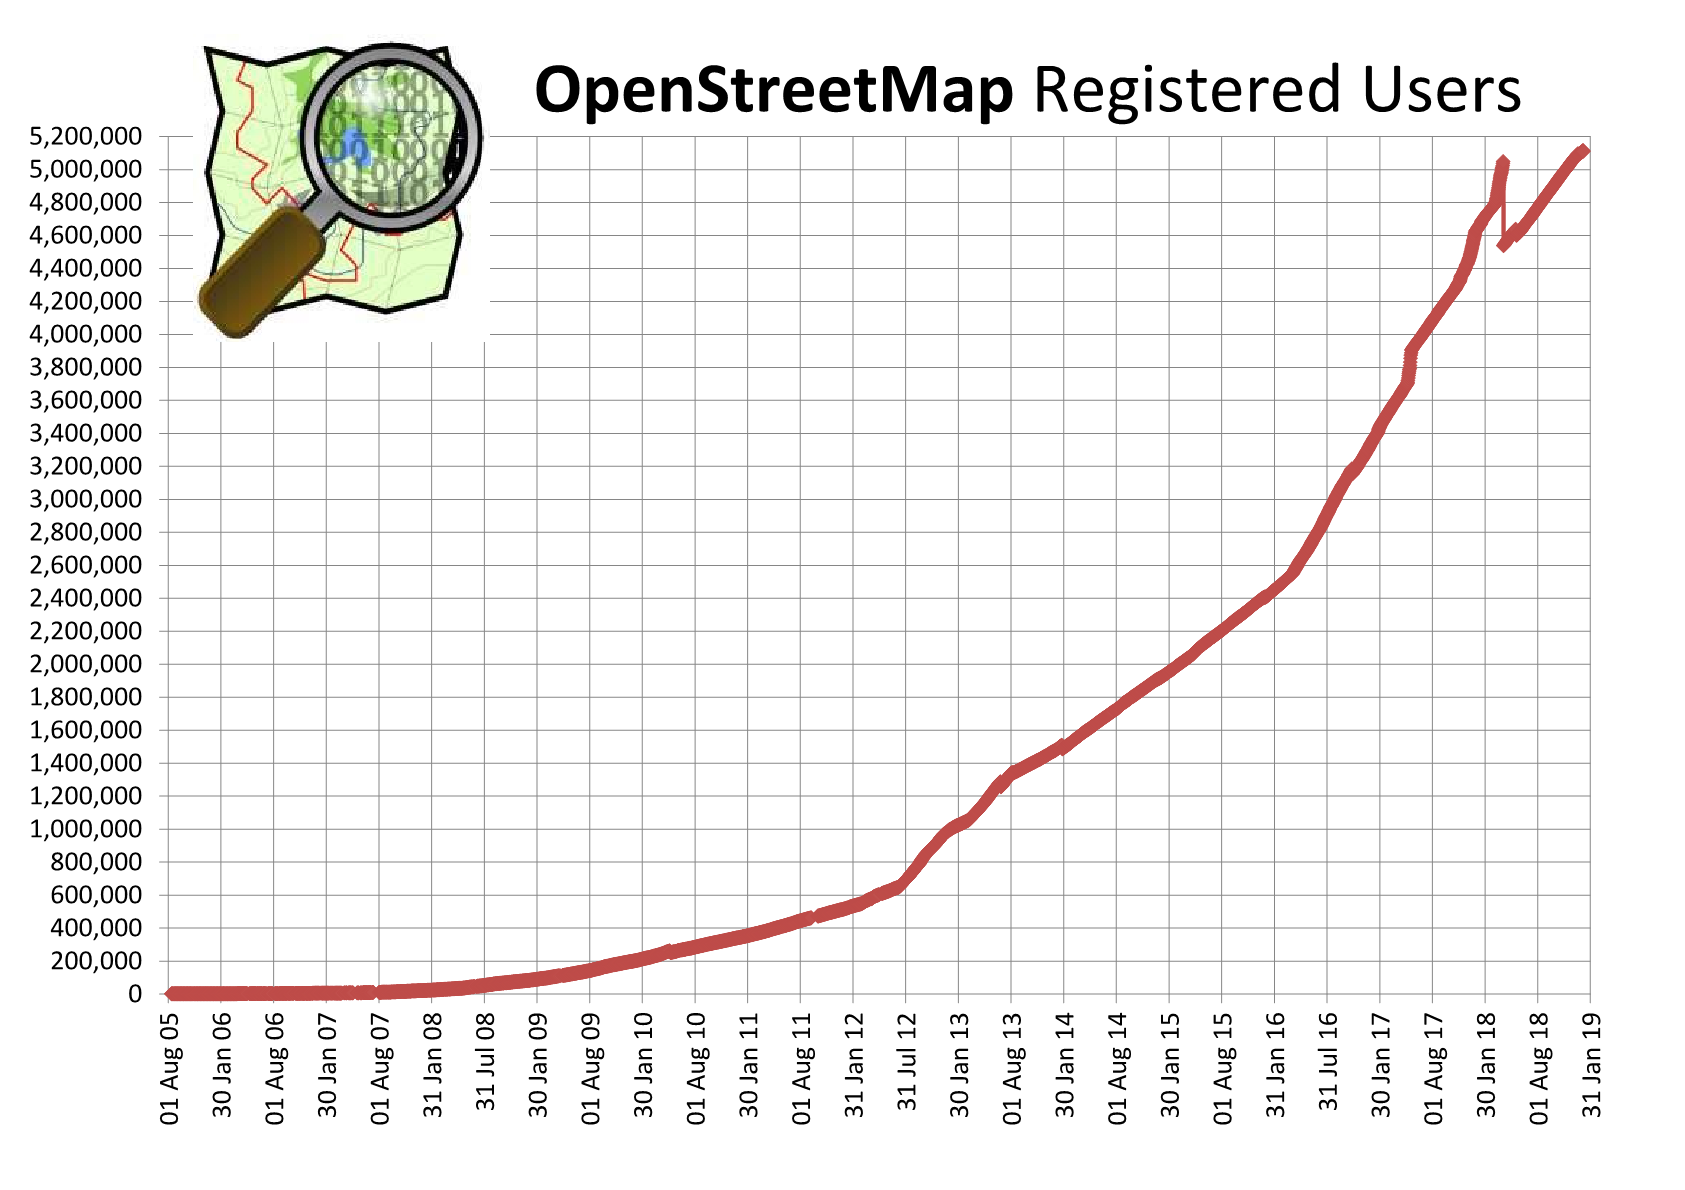
\includegraphics[width=\textwidth,height=\textheight,keepaspectratio]{images/Osmdbstats1_users.png}
		\end{center}
	\end{frame}

	\begin{frame}
		\begin{center}
			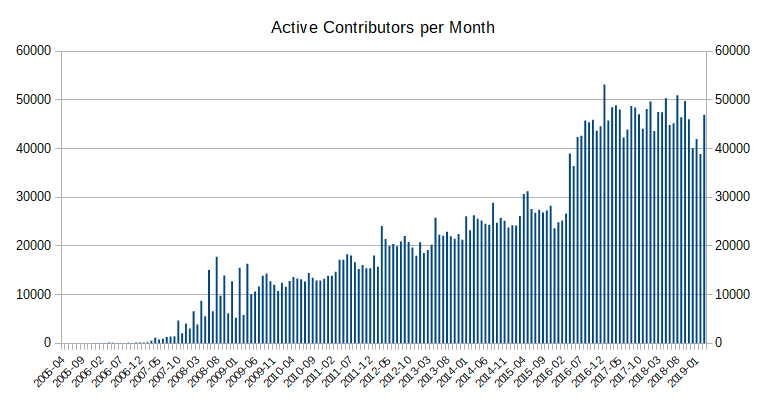
\includegraphics[width=\textwidth,height=\textheight,keepaspectratio]{images/Active_contributors_month.png}
		\end{center}
	\end{frame}
	
	\begin{frame}
		\begin{center}
			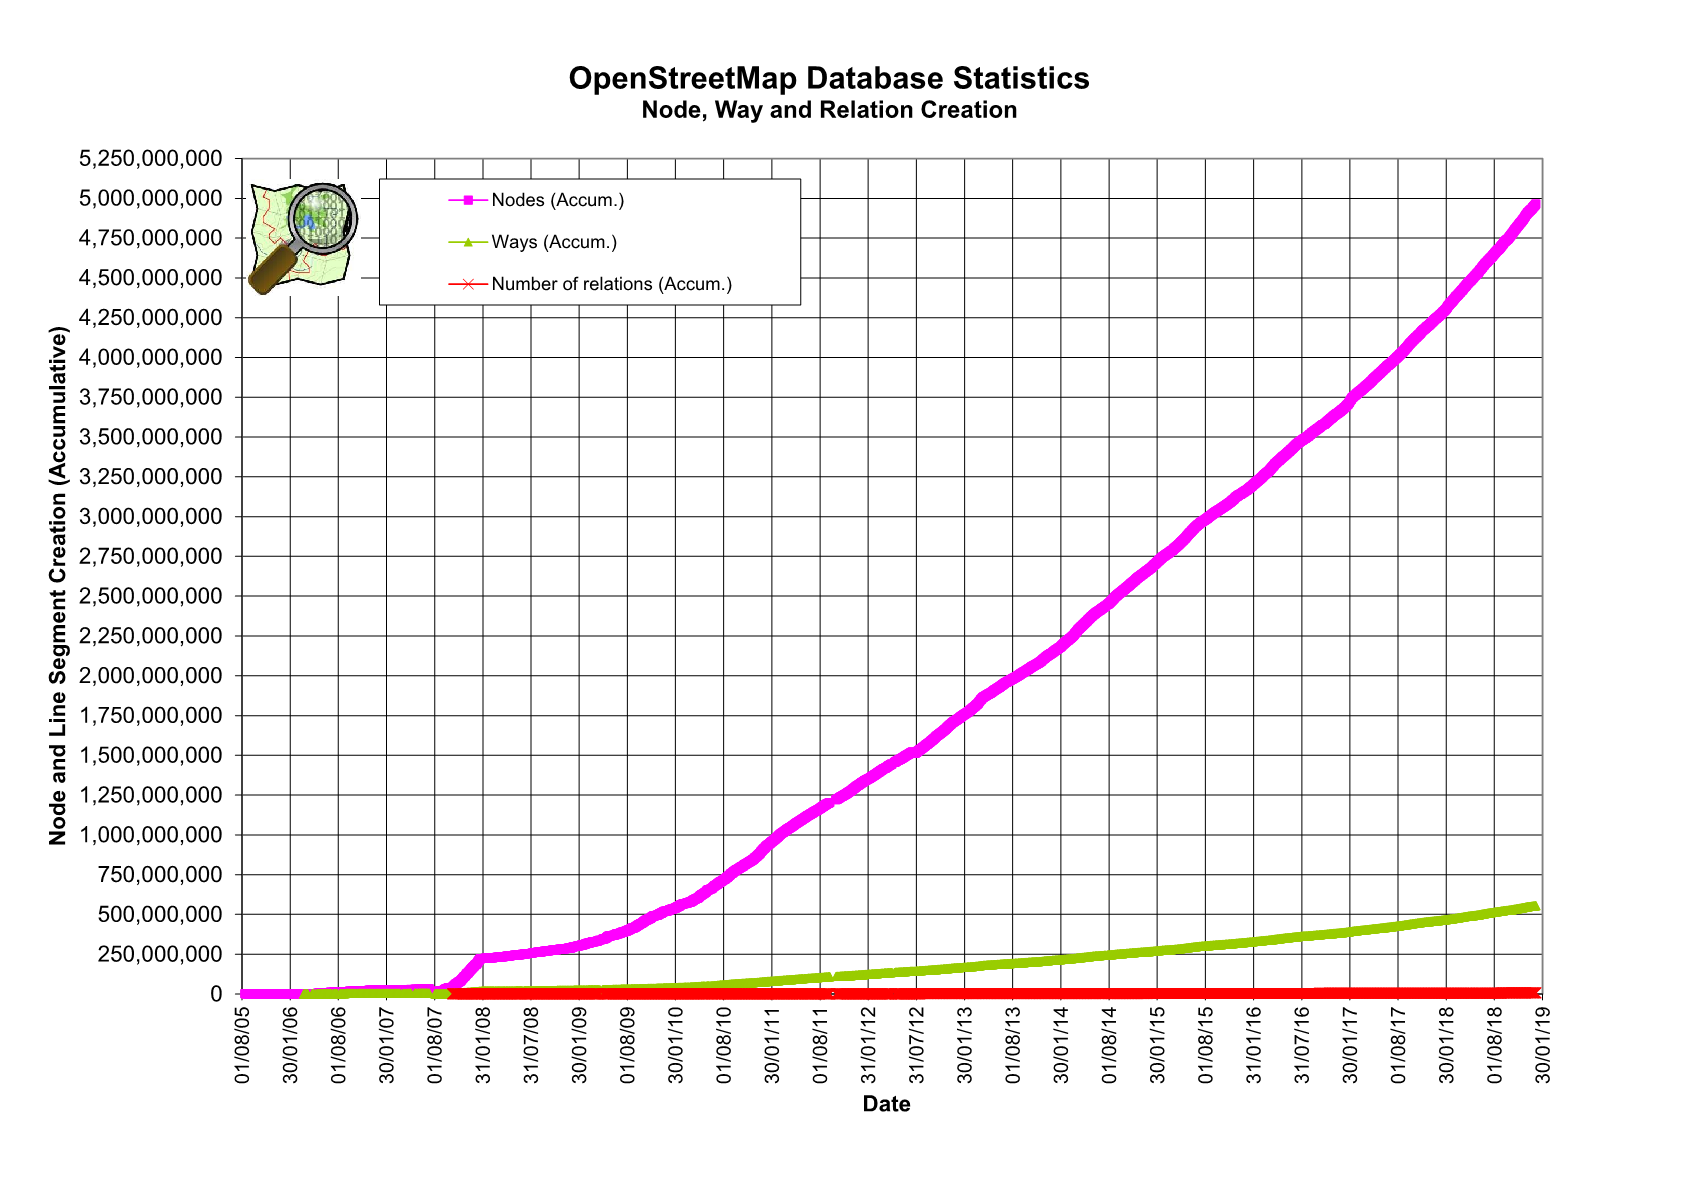
\includegraphics[width=\textwidth,height=\textheight,keepaspectratio]{images/Osmdbstats2.png}
		\end{center}
	\end{frame}
	
	\begin{frame}
		\begin{center}
			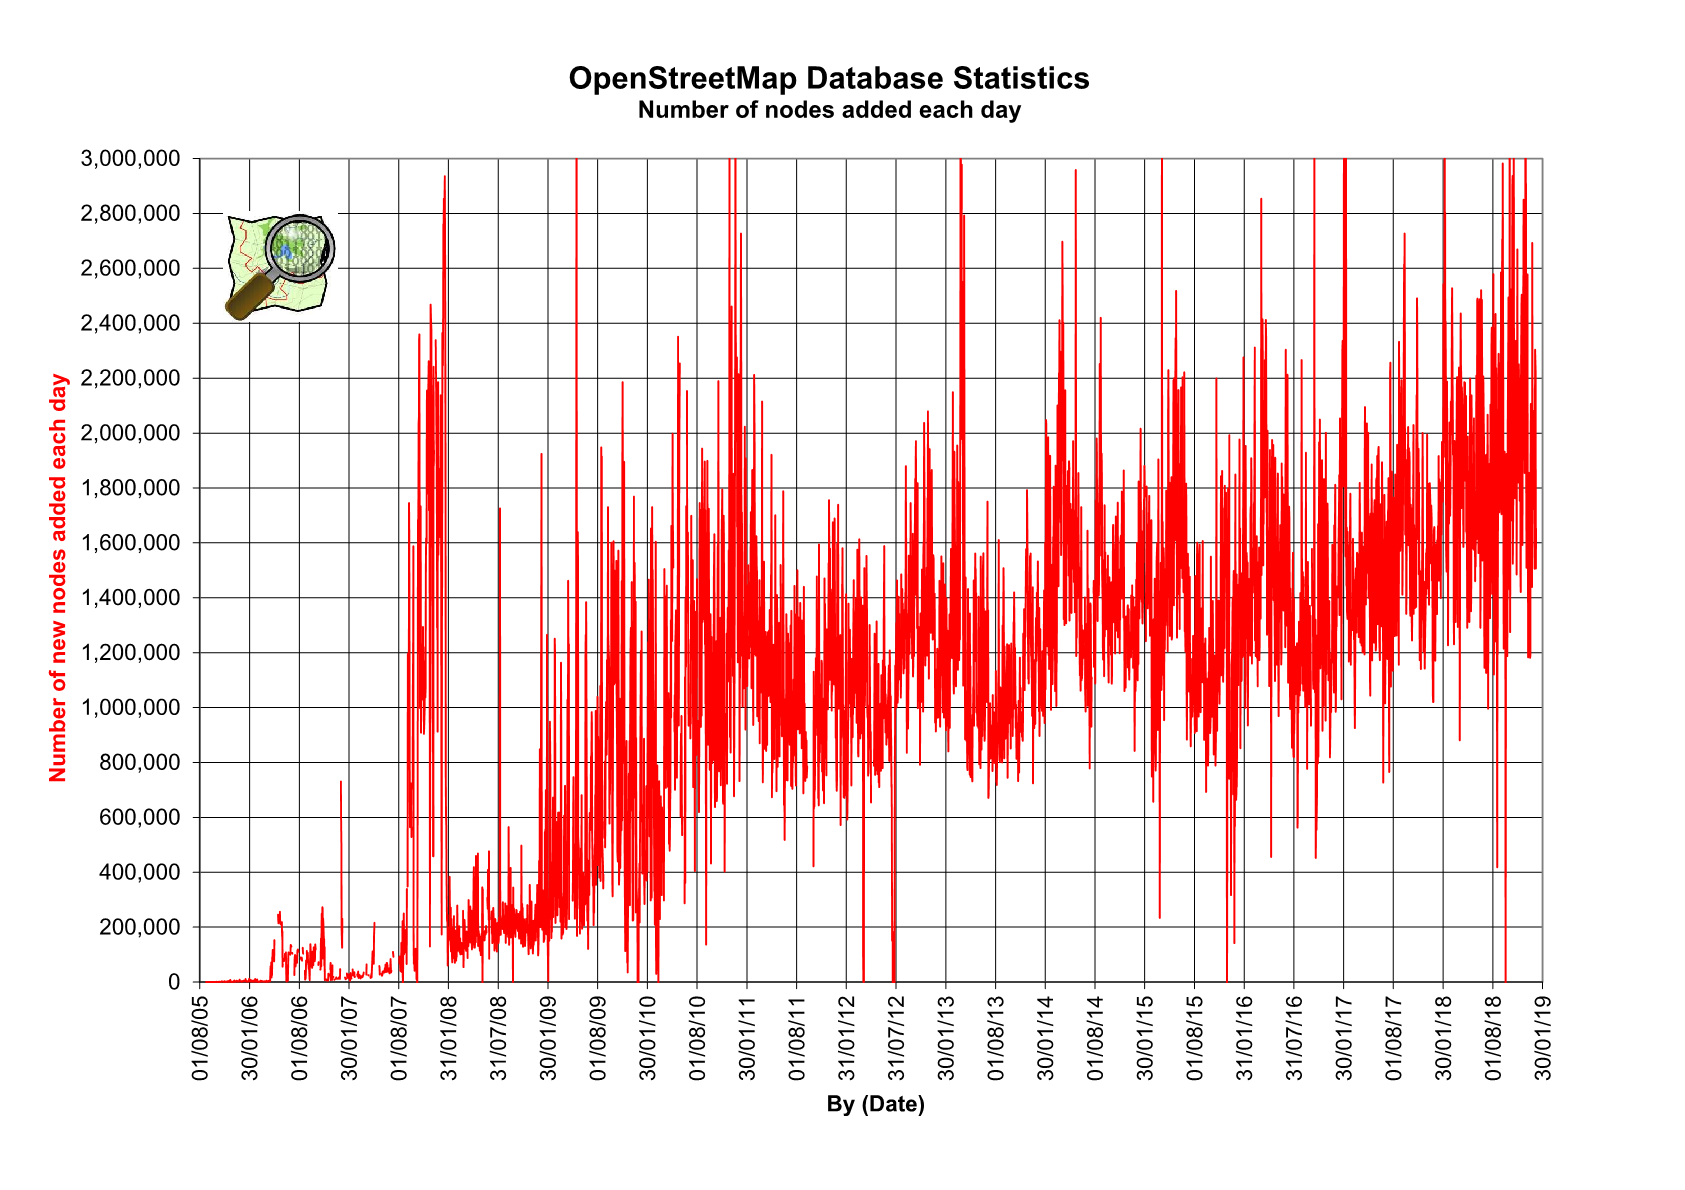
\includegraphics[width=\textwidth,height=\textheight,keepaspectratio]{images/Osmdbstats7A.png}
		\end{center}
	\end{frame}
	
	\begin{frame}
		\begin{center}
			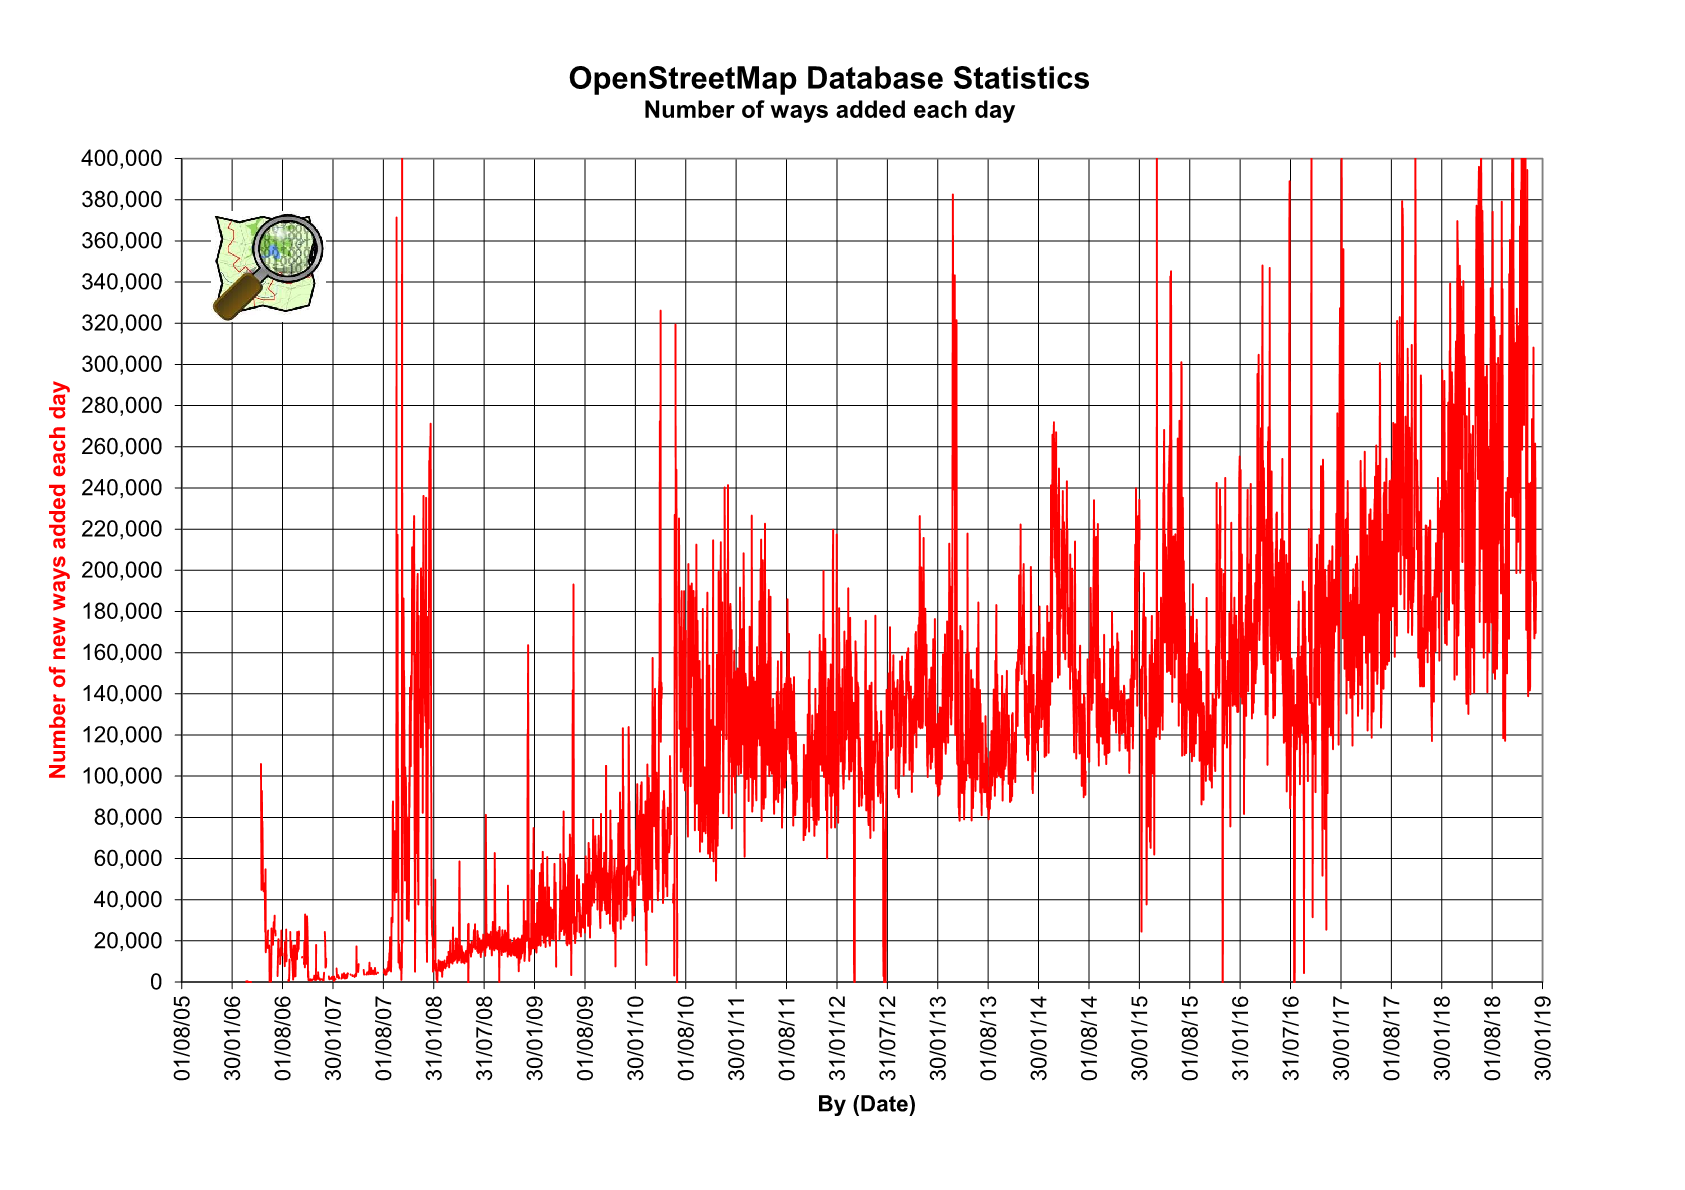
\includegraphics[width=\textwidth,height=\textheight,keepaspectratio]{images/Osmdbstats7B.png}
		\end{center}
	\end{frame}

	\subsection{Community}

	\begin{frame}{What is done?}
		\begin{itemize}
			\item developing software and tools
			\item actual mapping
			\item creating and maintaining documentation
			\item doing public relations activities
		\end{itemize}
	\end{frame}

	\begin{frame}{How is it done?}
		\begin{itemize}
		\item going outside collecting information
		\item using imagery services
		\item meet other mappers
		\item participating in a mapathon
		\end{itemize}
	\end{frame}

	\section{The data}
	
	\subsection{Node}
	
	\begin{frame}
		\begin{itemize}
			\item single location on map
		\end{itemize}
		
		\vfill
		
		\begin{center}
			\begin{minipage}[b][0.6\textheight][c]{0.2\linewidth}
				\centering
				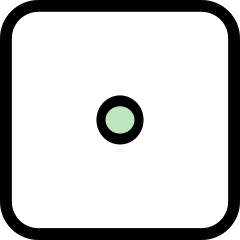
\includegraphics[width=0.5\linewidth,height=0.5\textheight,keepaspectratio]{images/240px-Mf_node.png}
			\end{minipage}
			\begin{minipage}[b][0.6\textheight][c]{0.4\linewidth}
				\centering
				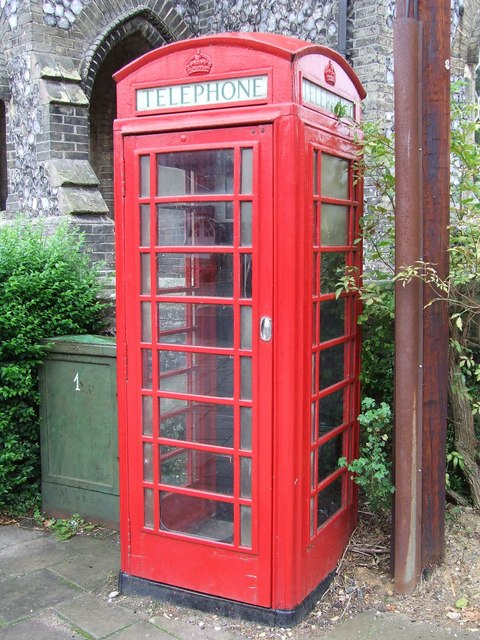
\includegraphics[width=0.8\linewidth,height=0.8\textheight,keepaspectratio]{images/red-telephone-box-uk.jpg}
			\end{minipage}
			\begin{minipage}[b][0.6\textheight][c]{0.3\linewidth}
				\texttt{amenity=telephone}\\
				\texttt{covered=booth}
				\begin{center}
					
\includegraphics[width=0.3\linewidth,height=0.3\textheight,keepaspectratio]{images/240px-Telephone.png}\\
					\vspace{0.25cm}
					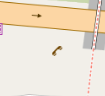
\includegraphics[width=0.8\linewidth,height=0.8\textheight,keepaspectratio]{images/telephone.png}
				\end{center}
			\end{minipage}
		\end{center}
	\end{frame}
		
	\subsection{Way}
	
	\begin{frame}
		\begin{itemize}
			\item line on map
			\item 2-2000 points per way
		\end{itemize}
		
		\vfill
		
		\begin{center}
			\begin{minipage}[b][0.6\textheight][c]{0.2\linewidth}
				\centering
				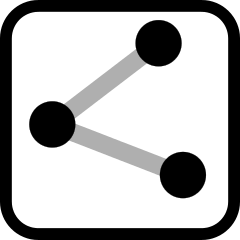
\includegraphics[width=0.5\linewidth,height=0.5\textheight,keepaspectratio]{images/240px-Mf_way.png}
			\end{minipage}
			\begin{minipage}[b][0.6\textheight][c]{0.4\linewidth}
				\centering
				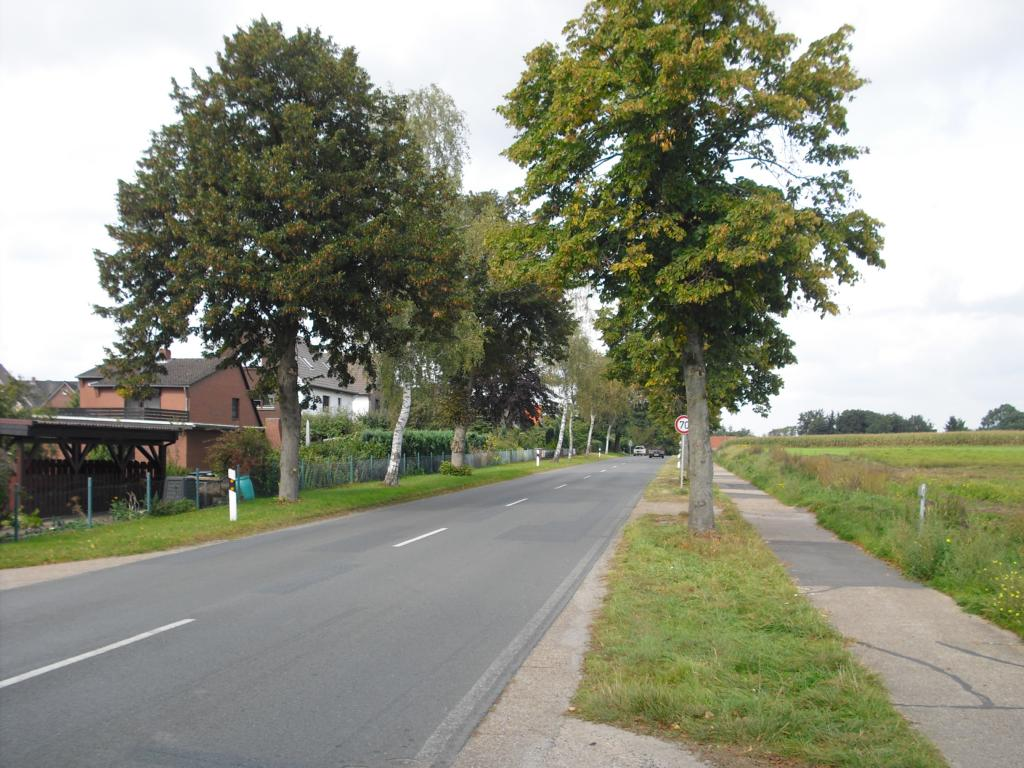
\includegraphics[width=0.8\linewidth,height=0.8\textheight,keepaspectratio]{images/Meyenburg-L134.jpg}
			\end{minipage}
			\begin{minipage}[b][0.6\textheight][c]{0.3\linewidth}
				\texttt{highway=secondary}
				\begin{center}
					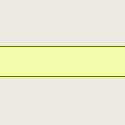
\includegraphics[width=0.3\linewidth,height=0.3\textheight,keepaspectratio]{images/Rendering-highway_secondary_neutral.png}\\
					\vspace{0.25cm}
				\end{center}
			\end{minipage}
		\end{center}
	\end{frame}
	
	\subsection{Relation}
	
	\begin{frame}
		\begin{itemize}
			\item combination of ways (e.g. to a bus route)
		\end{itemize}
		
		\vfill
		
		\begin{center}
			\begin{minipage}[b][0.6\textheight][c]{0.15\linewidth}
				\centering
				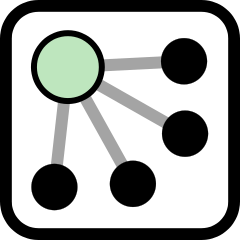
\includegraphics[width=0.5\linewidth,height=0.5\textheight,keepaspectratio]{images/240px-Mf_Relation.png}
			\end{minipage}
			\begin{minipage}[b][0.6\textheight][c]{0.5\linewidth}
				\centering
				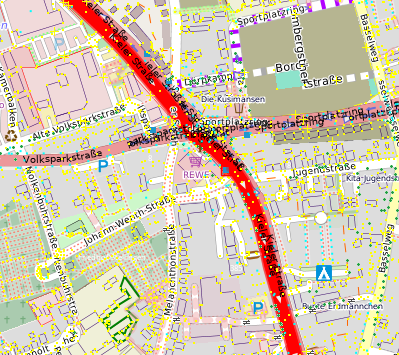
\includegraphics[width=0.8\linewidth,height=0.8\textheight,keepaspectratio]{images/relations_example.png}
			\end{minipage}
			\begin{minipage}[b][0.6\textheight][c]{0.3\linewidth}
				\texttt{type=route}\\
				\texttt{route=bus}\\
				\texttt{name=MetroBus 4}\\
				\texttt{ref=4}\\
				\texttt{from=Wildacker}\\
				\texttt{to=Brandstwiete}
			\end{minipage}
		\end{center}
	\end{frame}
	
	% TODO: Add real closed ways?
			
	\subsection{Area}
	
	\begin{frame}
		\begin{itemize}
			\item basically a closed way
		\end{itemize}
		
		\vfill
		
		\begin{center}
			\begin{minipage}[b][0.6\textheight][c]{0.2\linewidth}
				\centering
				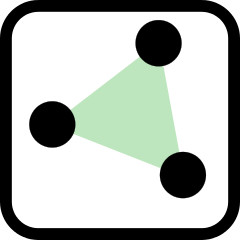
\includegraphics[width=0.5\linewidth,height=0.5\textheight,keepaspectratio]{images/240px-Mf_area.png}
			\end{minipage}
			\begin{minipage}[b][0.6\textheight][c]{0.4\linewidth}
				\centering
				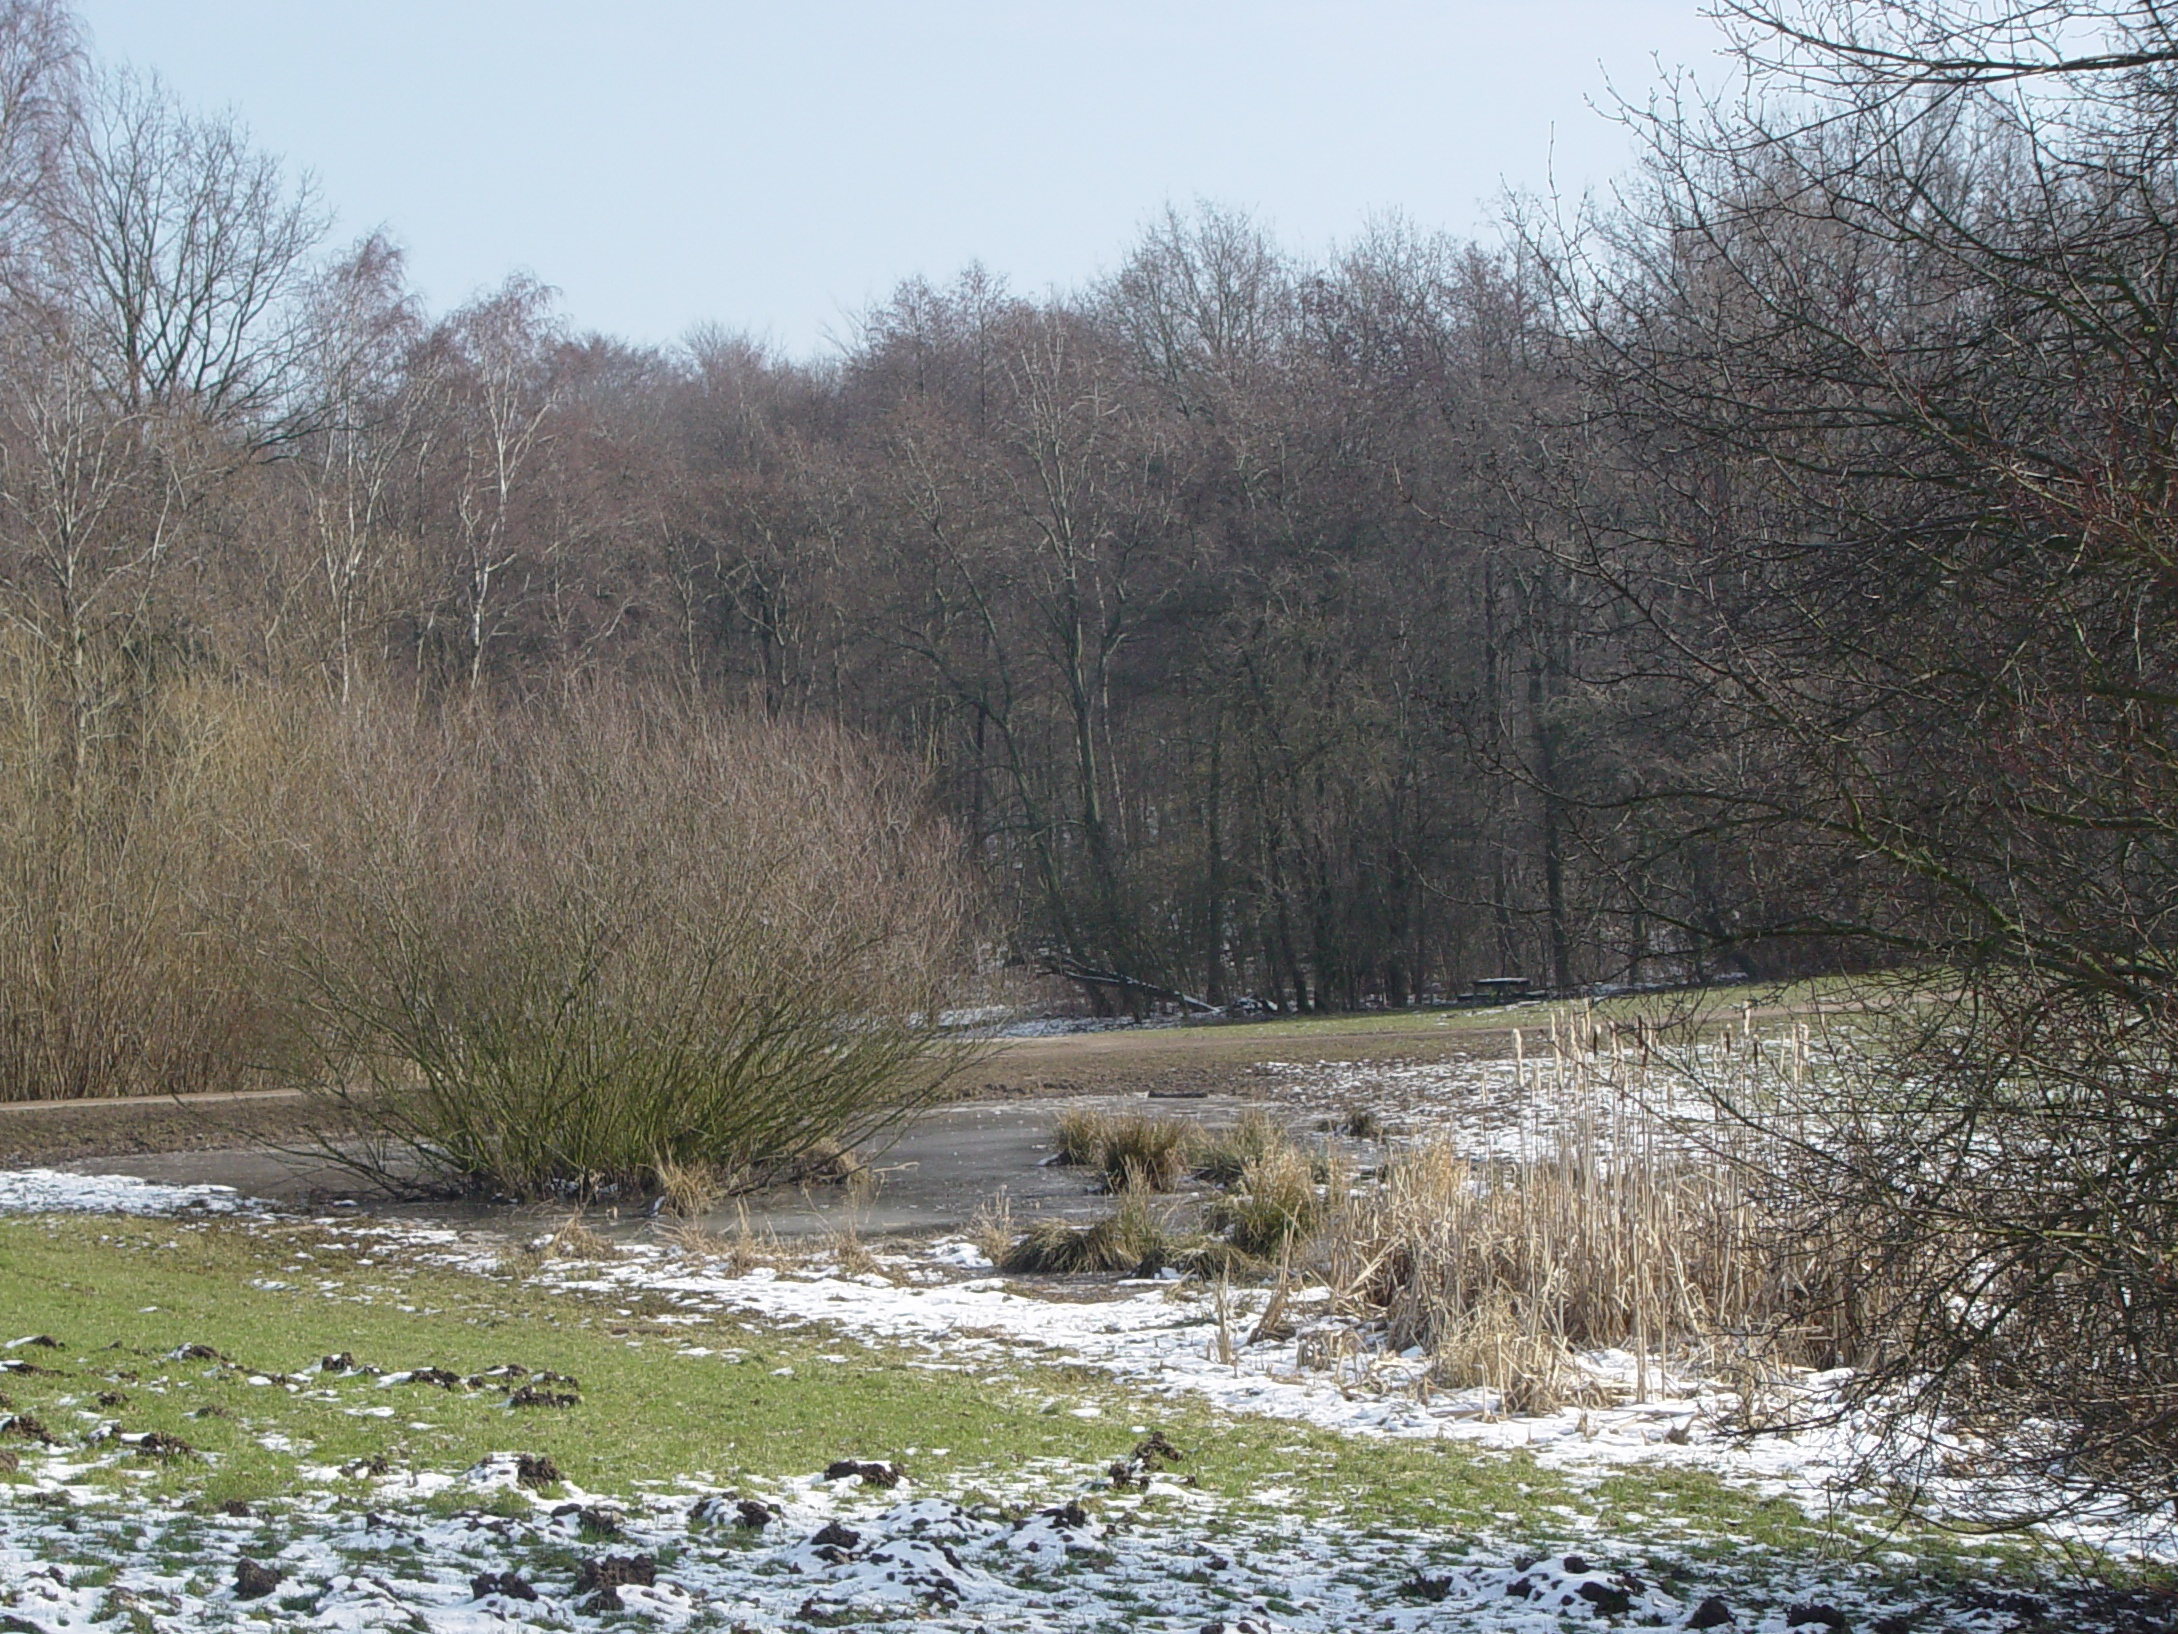
\includegraphics[width=0.8\linewidth,height=0.8\textheight,keepaspectratio]{images/Stellinger_Feldmark_ESE_01.JPG}
			\end{minipage}
			\begin{minipage}[b][0.6\textheight][c]{0.3\linewidth}
				\texttt{landuse=forest}\\
				\texttt{leaf\_type=broadleaved}
				\begin{center}
					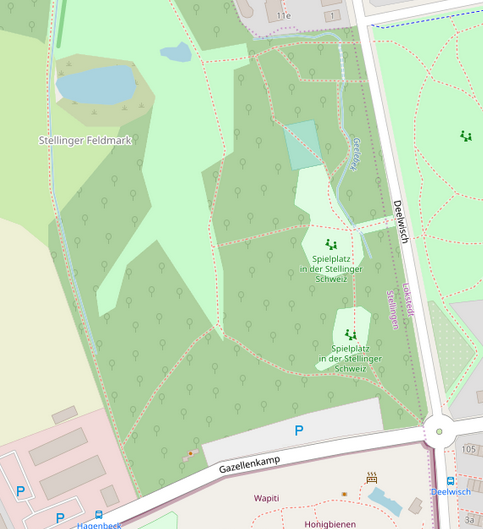
\includegraphics[width=\linewidth,height=\textheight,keepaspectratio]{images/forest.png}
				\end{center}
			\end{minipage}
		\end{center}
	\end{frame}
				
	\subsection{Multipolygon}
	
	\begin{frame}
		\begin{itemize}
			\item basically a polygon with polygons inside
			\item role \texttt{inner} and \texttt{outer}
		\end{itemize}
		
		\vfill
		
		\begin{center}
			\begin{minipage}[b][0.6\textheight][c]{0.2\linewidth}
				\centering
				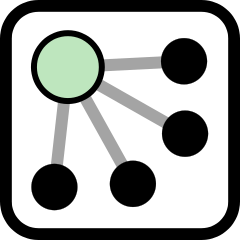
\includegraphics[width=0.5\linewidth,height=0.5\textheight,keepaspectratio]{images/240px-Mf_Relation.png}
			\end{minipage}
			\begin{minipage}[b][0.6\textheight][c]{0.4\linewidth}
				\centering
				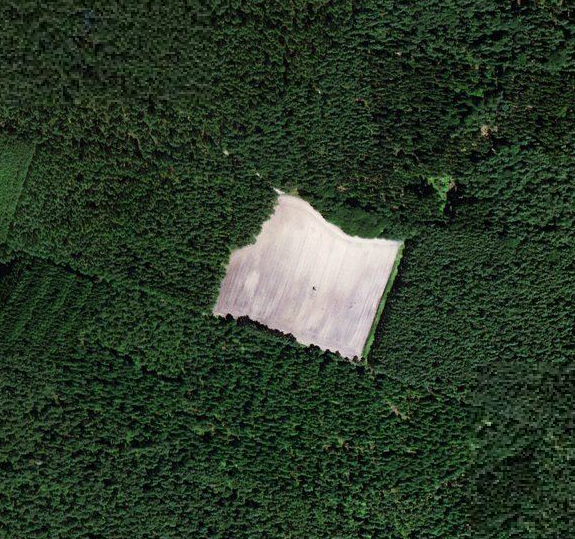
\includegraphics[width=0.8\linewidth,height=0.8\textheight,keepaspectratio]{images/multipolygon.png}
			\end{minipage}
			\begin{minipage}[b][0.6\textheight][c]{0.3\linewidth}
				\texttt{landuse=farmland}
				\begin{center}
					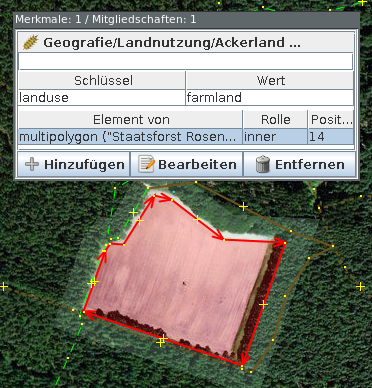
\includegraphics[width=\linewidth,height=\textheight,keepaspectratio]{images/multipolygon_josm.png}
				\end{center}
			\end{minipage}
		\end{center}
	\end{frame}

	\section{Contributing to OSM}
	
	\subsection{Trace aerial imagery}
	
	\subsection{Go outside}
	
	\subsection{Report errors}
	
	\subsection{Socialize}
	
	\section{Editors}
	
	\subsection{iD}
	
	\subsection{JOSM}
	
	\section{Hands-On}
\end{document}












